\documentclass[12pt]{article}
\setlength\parindent{0pt}
\usepackage{fullpage}
\usepackage{amsmath}
\usepackage{graphicx}
\usepackage[left=2cm, right=2cm, top=1.5cm, bottom=1cm]{geometry}
\setlength{\parskip}{4mm}
\def\LL{\left\langle}   % left angle bracket
\def\RR{\right\rangle}  % right angle bracket
\def\LP{\left(}         % left parenthesis
\def\RP{\right)}        % right parenthesis
\def\LB{\left\{}        % left curly bracket
\def\RB{\right\}}       % right curly bracket
\def\PAR#1#2{ {{\partial #1}\over{\partial #2}} }
\def\PARTWO#1#2{ {{\partial^2 #1}\over{\partial #2}^2} }
\def\PARTWOMIX#1#2#3{ {{\partial^2 #1}\over{\partial #2 \partial #3}} }
\newcommand{\BE}{\begin{displaymath}}
\newcommand{\EE}{\end{displaymath}}
\newcommand{\BNE}{\begin{equation}}
\newcommand{\ENE}{\end{equation}}
\newcommand{\BEA}{\begin{eqnarray}}
\newcommand{\EEA}{\nonumber\end{eqnarray}}
\newcommand{\EL}{\nonumber\\}
\newcommand{\la}[1]{\label{#1}}
\newcommand{\ie}{{\em i.e.\ }}
\newcommand{\eg}{{\em e.\,g.\ }}
\newcommand{\cf}{cf.\ }
\newcommand{\etc}{etc.\ }
\newcommand{\Tr}{{\rm tr}}
\newcommand{\etal}{{\it et al.}}
\newcommand{\OL}[1]{\overline{#1}\ } % overline
\newcommand{\OLL}[1]{\overline{\overline{#1}}\ } % double overline
\newcommand{\OON}{\frac{1}{N}} % "one over N"
\newcommand{\OOX}[1]{\frac{1}{#1}} % "one over X"



\begin{document}
\pagenumbering{gobble}
\Large
\centerline{\sc{Recitation Questions}}
\normalsize
\centerline{\sc{5 March}}

A penguin slides down a frictionless icy hill; the hill is inclined at an angle $\theta$. In this problem, you will 
calculate the penguin's acceleration. However, I want you to do it two different ways, using two different coordinate systems.

First, solve the problem using the conventional coordinate system, where $x$ is horizontal and $y$ is vertical. As usual, take the following steps:

a) Draw a cartoon of the problem, and label your coordinate system.

\vspace{2in}


b) Draw a force diagram for the penguin. 

\vspace{2in}

c) Write down Newton's second law in both directions -- that is, $\sum F_x = ma_x$ and $\sum F_y = ma_y$. If you have any forces that don't lie along the $x$ or $y$ directions, use trigonometry to break them into components.

\vspace{2in}
\newpage
d) This will result in two equations with three unknowns: $a_x$, $a_y$, and $F_N$. However, in this problem, $a_x$ and $a_y$ are related. What is their relation? This should reduce you to two equations and two unknowns; write them below.
\vspace{3in}

e) Solve those equations to find the acceleration of the penguin. Use trigonometry to find the magnitude of $\vec a$.

\newpage
Now you will solve the problem again using a rotated coordinate system, where $x$ is the direction parallel to the hill and $y$ is the direction perpendicular to it. Again:

a) Draw a cartoon of the problem, and label your coordinate system. 

\vspace{2in}

b) Draw a force diagram for the penguin. (Draw this one large, since you will need to construct a right triangle 
with one of the forces as its hypotenuse to break it into components.) 

\vspace{3in}

c) Write down Newton's second law in both directions -- that is, $\sum F_x = ma_x$ and $\sum F_y = ma_y$. 
If you have any forces that don't lie along the $x$ or $y$ directions, use trigonometry to break them into components.
This will require some thought: you will need to figure out the components of the 
penguin's weight in the $x$ and $y$ directions. Call over your TA or coach to check your work when you are done.

\vspace{3in}
\newpage

d) This will result in two equations with three unknowns: $a_x$, $a_y$, and $F_N$. However, a little thought will
tell you what one of these is. What is it? This should reduce you to two equations and two unknowns; write them below.

\vspace{2in}

e) Solve those equations to find the acceleration of the penguin.

\vspace{2in}

f) Discuss the difference in the two approaches. In one, you aligned your coordinate system with gravity, and in the other, you aligned your coordinate system with the direction that you knew the penguin would accelerate in. Which was easier? Which 
should you adopt for future problems? Invite your TA or coach over to join your conversation.

\newpage
\begin{minipage}{0.7\textwidth}
Two weights of mass $m_1$ and $m_2$ are attached to either end of a string. This string is passed over a light frictionless pulley, as shown in the image.
Clearly the heavier mass will go down and the lighter one will go up, but at what rate? In this problem, you will calculate their acceleration.
\end{minipage} \hfill
\begin{minipage}{0.3\textwidth}
\begin{center}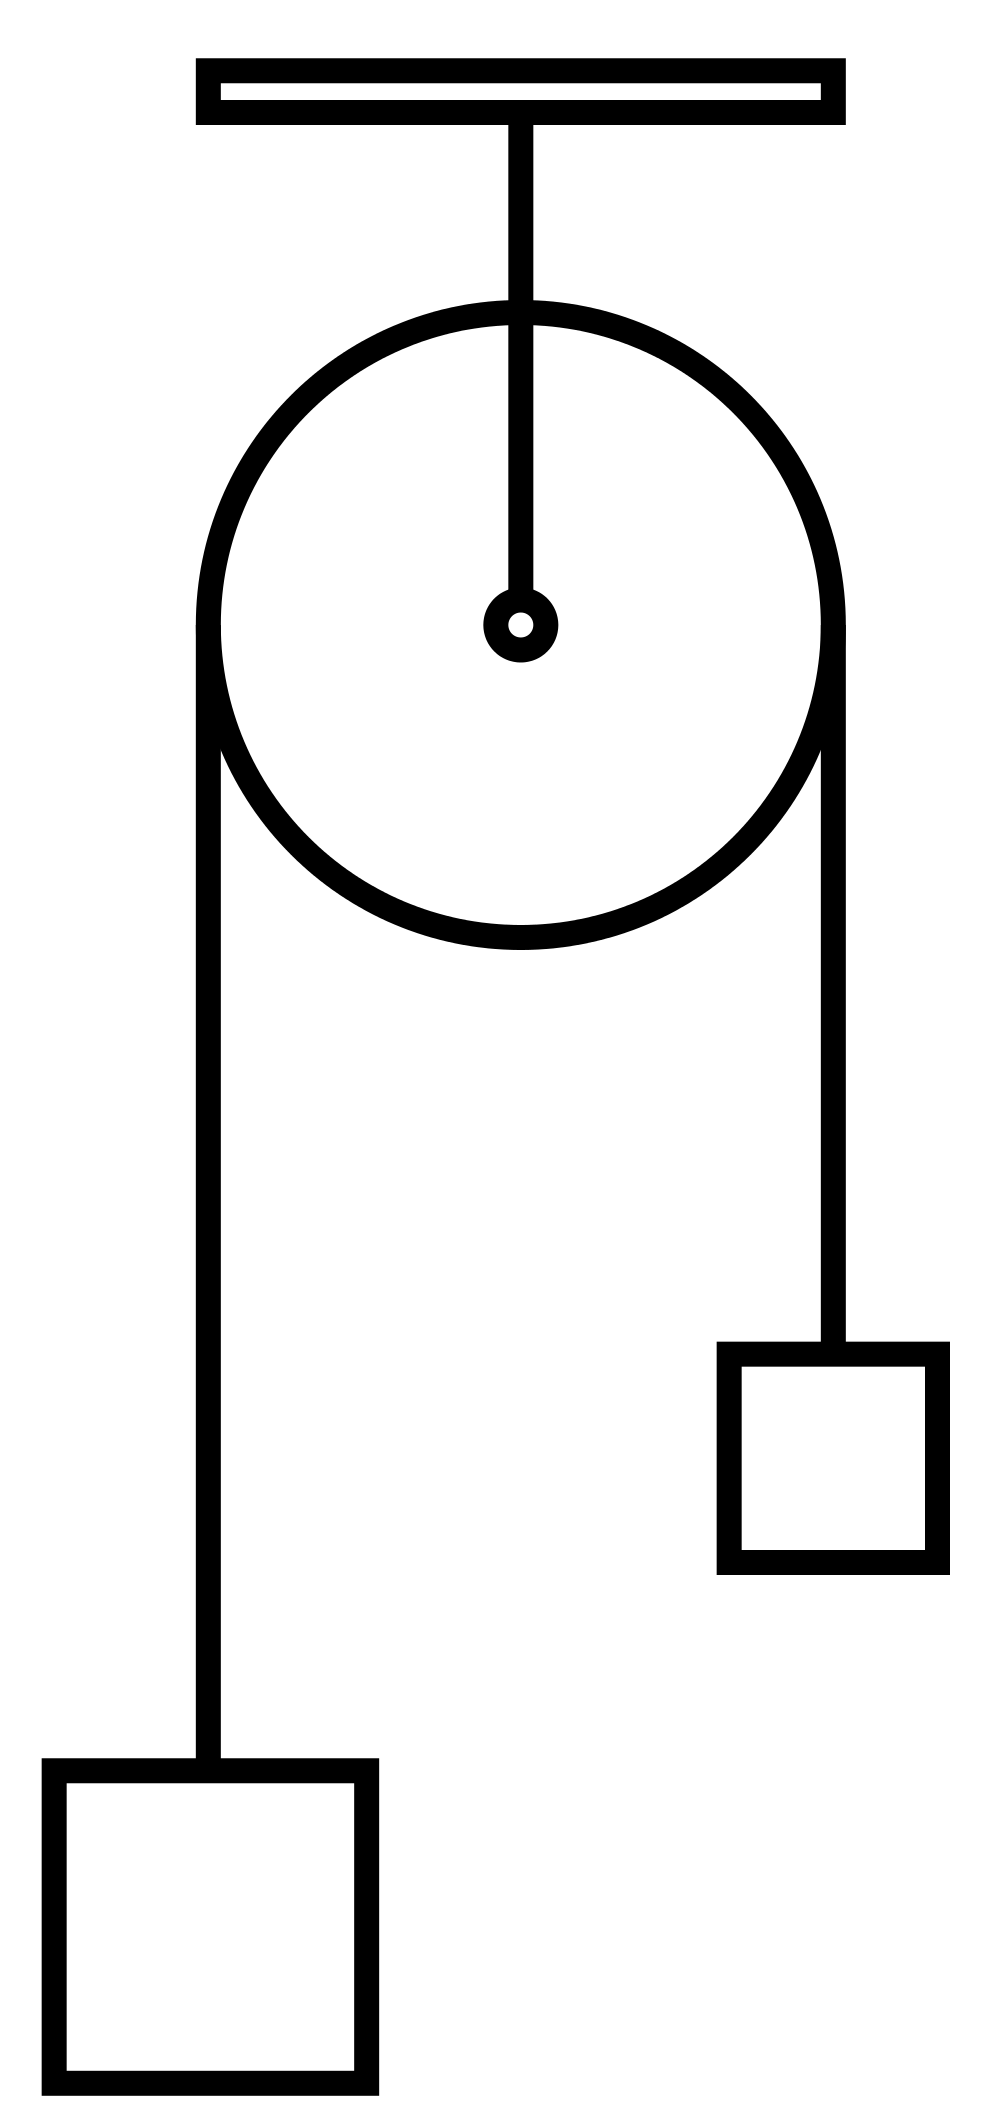
\includegraphics[width=0.5\textwidth]{atwood.png}
\end{center}
\end{minipage} \hfill

a) What do you expect the system to do if one of the masses is much heavier than the other? What do you expect if the
two masses are equal?

\vspace{1in}

b) Draw force diagrams for both objects. Label your choice of coordinate system separately for each object -- you don't have to choose the same coordinate system for each! 

\vspace{2in}

c) State Newton's law for both objects. Note that their accelerations aren't necessarily the same, depending on your choice of coordinate system, so you should introduce separate variables $a_1$ and $a_2$ for both. The tension forces
{\it are} the same.

\newpage

d) Since you have two objects, you have two copies of Newton's law. However, you have three unknowns: $T$, $a_1$, and $a_2$. What other statement can you make about the accelerations that lets you solve the system?

\vspace{3in}

e) Actually solve the system, giving values of $a_1$ and $a_2$ in terms of $m_1$, $m_2$, and $g$. Then, translate 
your expressions for $a_1$ and $a_2$ into words. (Your TA and coaches can help with this.) Does your result make sense?
Does it agree with your predictions in part (a)? 

\end{document}
